\documentclass{article}
\usepackage{graphicx}
\usepackage[margin=0.85in]{geometry}
\title{Problem 2(b): Visualization and Error Analysis}
\author{}
\date{}
\begin{document}
\maketitle

\section{Training loss}
The curve uses the epoch-mean training loss already stored in \texttt{outputs/segmentation3d/history.csv} for the Problem 2(a) run (\texttt{best.pt}, epoch 170). Each point is the mean of the iteration losses in that epoch. The total is CE + Dice with both weights equal to 1. CE and Dice loss are plotted as well. The curves are the raw epoch values, with no smoothing and no resampling.

\begin{figure}[ht]
\centering
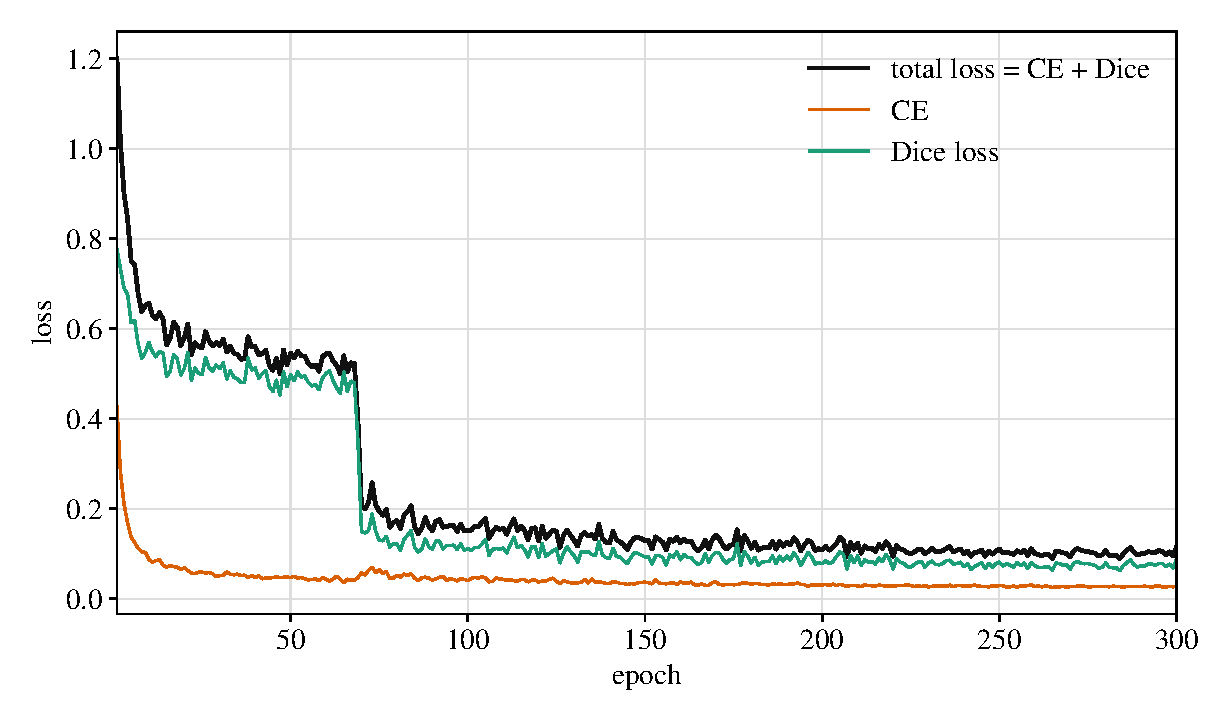
\includegraphics[width=\textwidth]{training_loss.pdf}
\caption{Training loss of the 3D U-Net. The black curve is the epoch-mean total loss, equal to CE + Dice. The orange and green curves are the CE and Dice components.}
\end{figure}

The epoch-mean total loss starts at 1.202 in epoch 1 (CE 0.426, Dice loss 0.776). It declines with visible epoch-to-epoch fluctuation, then the recorded mean falls from 0.523 at epoch 68 to 0.207 at epoch 70. The log does not by itself identify the cause of that step. By epoch 100 the total is 0.152 (CE 0.040, Dice loss 0.111). The lowest epoch mean is 0.089 at epoch 265. From epoch 200 through epoch 300 the total stays between 0.089 and 0.137, and epoch 300 ends at 0.116. After epoch 70 the Dice component remains larger than CE, so the late total tracks the Dice loss.

\section{Four test cases}
The four cases are distinct members of the official test split. Predictions are the raw full-volume argmax masks saved by Problem 2(a) (\texttt{postprocess: none}), restored on the original \((X,Y,Z)\) grid. No connected-component filter was added. Dice and HD95 below are the full-volume values and match \texttt{per\_case\_metrics.csv}. HD95 is in voxels: the NRRD \texttt{space directions} have unit length and the files contain no \texttt{space units}.

\begin{figure}[ht]
\centering
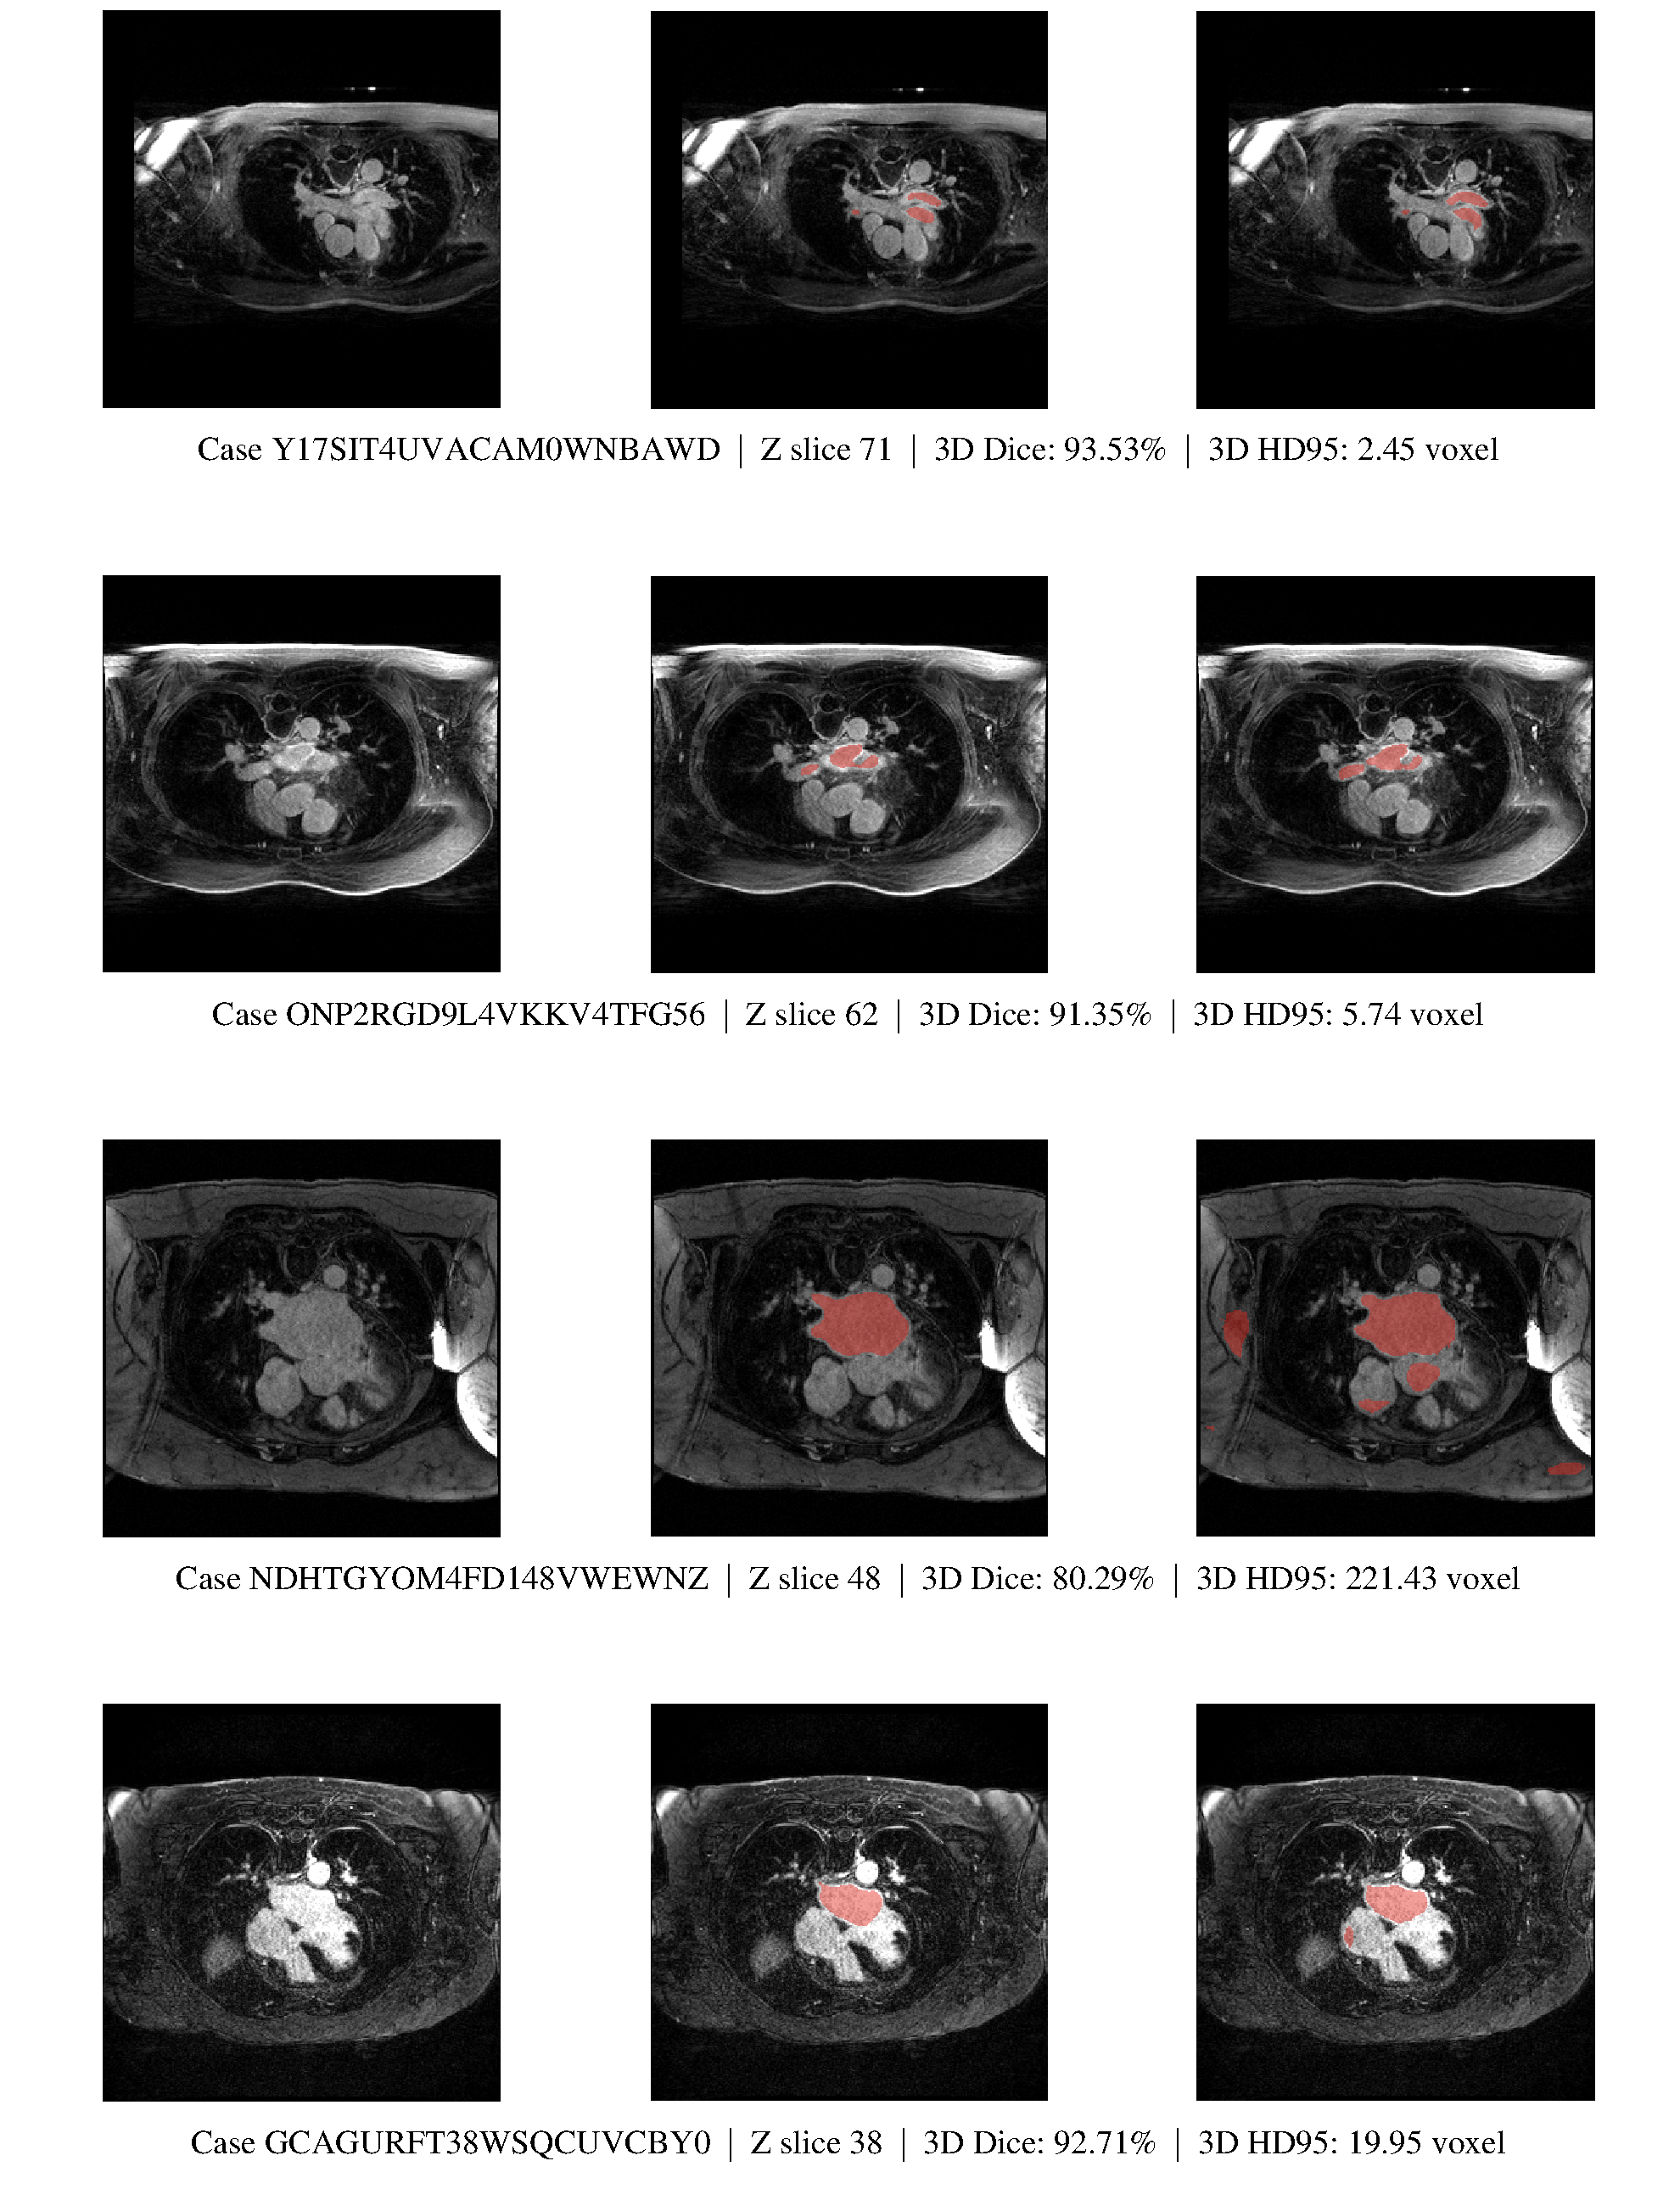
\includegraphics[width=0.96\textwidth]{test_cases_4x3.pdf}
\caption{One axial (Z) slice from each of four test cases. Columns are the MRI, the same MRI with the ground-truth mask, and the same MRI with the predicted mask. The foreground color and the grayscale window are shared within a row. The printed Dice and HD95 are 3D volume scores, not scores of the displayed slice.}
\end{figure}

\begin{table}[ht]
\centering
\resizebox{\textwidth}{!}{%
\begin{tabular}{llrrrr}
\hline
Case & Role & Z slice & 3D Dice (\%) & 3D HD95 (voxel) & Volume FP / FN \\
\hline
Y17SIT4UVACAM0WNBAWD & high Dice, low HD95 & 71 & 93.53 & 2.45 & 15073 / 3104 \\
ONP2RGD9L4VKKV4TFG56 & Dice near the test median & 62 & 91.35 & 5.74 & 18596 / 14620 \\
NDHTGYOM4FD148VWEWNZ & low Dice & 48 & 80.29 & 221.43 & 168365 / 10174 \\
GCAGURFT38WSQCUVCBY0 & Dice still reasonable, HD95 elevated & 38 & 92.71 & 19.95 & 12233 / 14650 \\
\hline
\end{tabular}}
\caption{Full-volume Dice and HD95 for the visualized test cases. FP and FN counts are also full-volume voxel counts. Slice-wise counts are in \texttt{selected\_cases\_metrics.csv} and are not a substitute for these 3D scores.}
\end{table}

\section{Error analysis}
The auxiliary overlay marks true positives in green, false positives in red, and false negatives in blue on the same slices. It is evidence for the notes below. It does not replace the 4$\times$3 figure, and a slice count is not the 3D score.

\begin{figure}[ht]
\centering
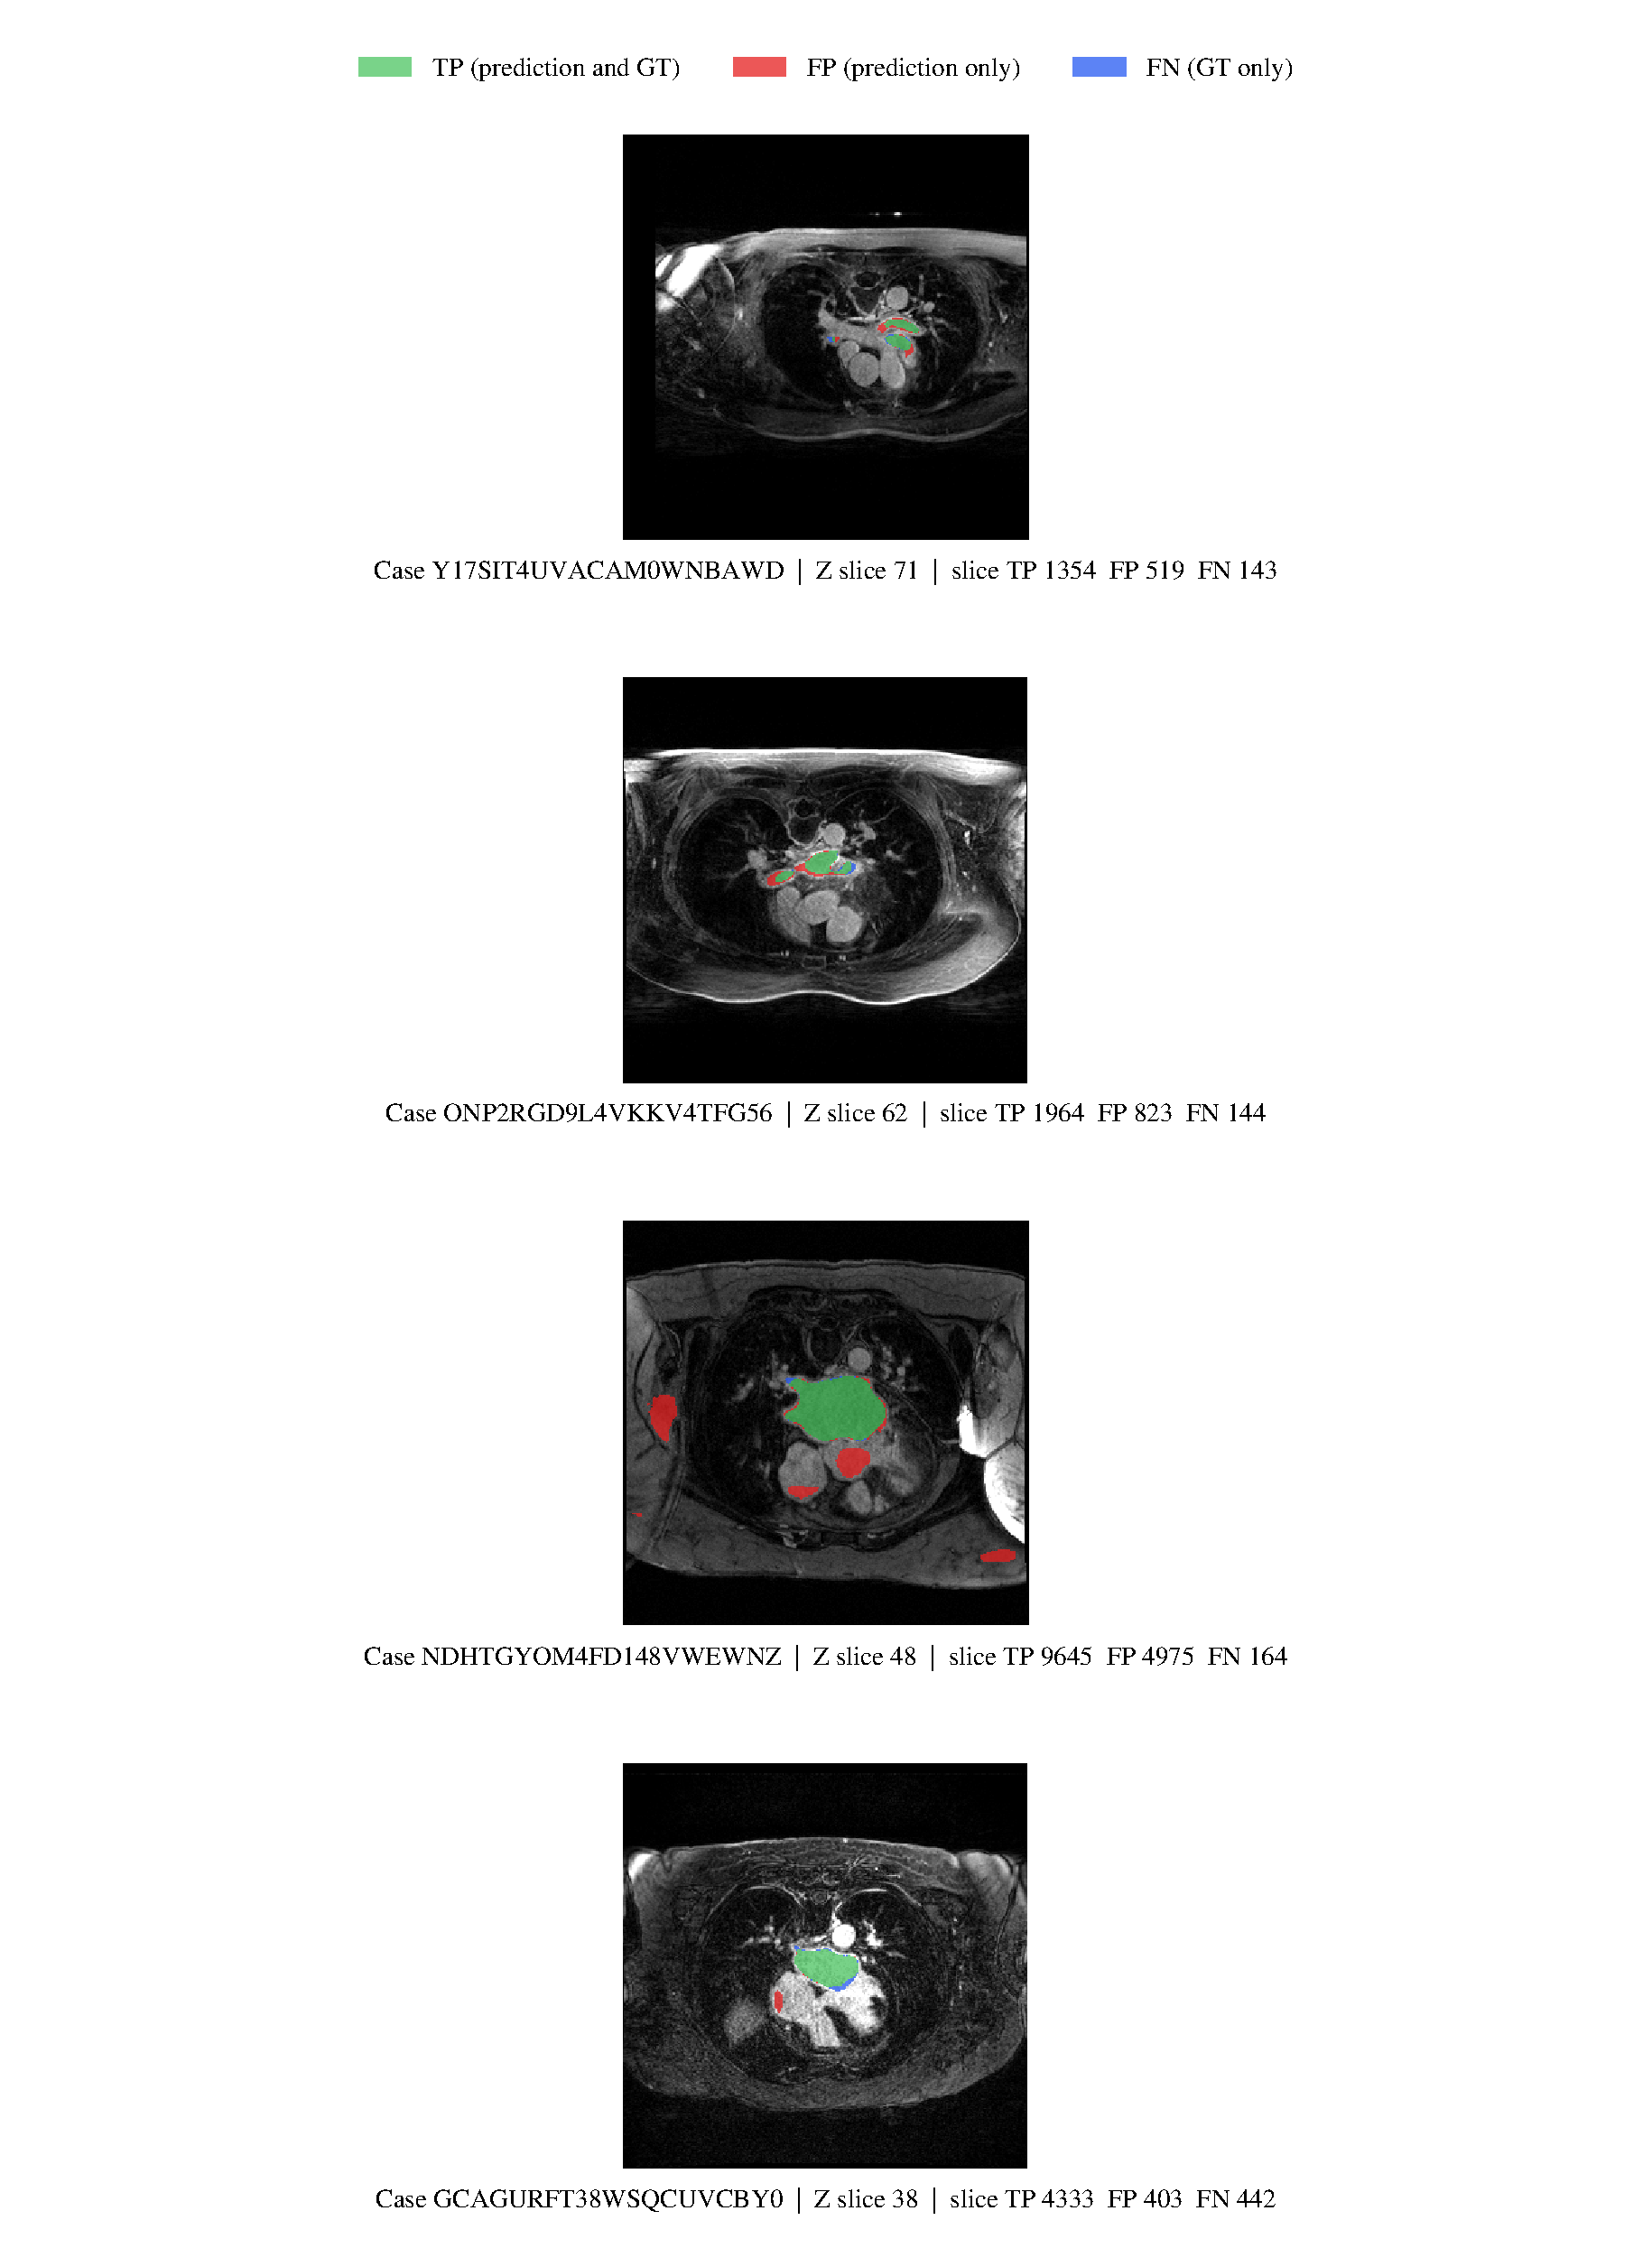
\includegraphics[width=0.48\textwidth]{test_cases_error_overlay.pdf}
\caption{Error overlay for the same four Z slices. Green is overlap, red is predicted foreground outside the ground truth, and blue is missed ground truth.}
\end{figure}

\paragraph{Y17SIT4UVACAM0WNBAWD.}
On Z slice 71 the error overlay shows a thin false-positive rim around the overlapped atrium and a small ground-truth focus that is only partly covered (TP 1354, FP 519, FN 143). The prediction is a single 26-connected component and it overlaps the ground truth, so this is a boundary mismatch rather than a detached false-positive island. Full-volume false positives (15073) exceed false negatives (3104); both reduce $|P \cap G|$ relative to $|P|+|G|$, but the overlap is still large enough for a 3D Dice of 93.53\%. HD95 stays 2.45 voxel because the surface deviations are short: the maximum surface distance is 10.49 voxel, and 0.003\% of surface points are farther than 10 voxels. Only 4.8\% of the HD95 tail lies on this slice, so the same kind of rim also occurs elsewhere in the volume.

\paragraph{ONP2RGD9L4VKKV4TFG56.}
On Z slice 62 the overlay shows added prediction on one side of the atrium and missed ground truth on another, with the center overlapped (TP 1964, FP 823, FN 144). Those voxels belong to the main component; this slice contains none of the three predicted components that miss the ground truth. Those components are 439 voxels at least 8.1 voxels from the ground truth (Z 68--73), 153 voxels at least 14.5 voxels from the ground truth (Z 66--70), plus one isolated voxel at Z 35 whose nearest ground-truth voxel is 236.8 voxels away. The isolated voxel is not on the displayed slice. It sets the maximum surface distance, but it is one of 42710 surface points, so it does not move the 95th percentile: 3D HD95 remains 5.74 voxel. Only 1.81\% of surface points are farther than 10 voxels, and 1.2\% of the HD95 tail is on this slice. Volume FP 18596 and FN 14620 are similar in count, and together they bring the 3D Dice to 91.35\%.

\paragraph{NDHTGYOM4FD148VWEWNZ.}
Z slice 48 shows the ground-truth atrium mostly covered (TP 9645, FN 164) and several red false-positive islands that do not overlap it. Of the 4975 false-positive voxels on this slice, 4591 lie in 6 components that have no ground-truth overlap anywhere; the rest are attached to the main prediction. Across the volume there are 10 such components. The largest has 55202 voxels and its nearest ground-truth voxel is 138.5 voxels away; 9 components are at least 50 voxels from the ground truth, while 1 component is closer than 20 voxels. That nearer component adds local false-positive volume, and the far islands place surface points hundreds of voxels away. Full-volume FP (168365) greatly exceeds FN (10174), which enlarges $|P|$ without a matching increase in $|P \cap G|$ and lowers the 3D Dice to 80.29\%. HD95 is 221.43 voxel. This slice contains only 3.0\% of the volume FP voxels and 2.8\% of the HD95 tail (the tail is heaviest on other Z slices, led by Z 46), so the islands visible here illustrate the failure but do not contain it.

\paragraph{GCAGURFT38WSQCUVCBY0.}
On Z slice 38 the main atrium is largely overlapped, with a false-negative rim, and a separate predicted island that does not meet the ground truth on this slice (TP 4333, FP 403, FN 442; 369 of the slice FP voxels belong to that island). In 3D the island is one component of 7371 voxels spanning Z 29--56, with no ground-truth overlap and a nearest ground-truth voxel 35.6 voxels away. It was not removed. Relative to the 170899 overlapping voxels, this extra region and the remaining boundary errors (volume FP 12233, FN 14650) leave the 3D Dice at 92.71\%. HD95 is still 19.95 voxel because the island's surface is far from the ground-truth surface, and 6.38\% of all surface points are farther than 10 voxels. Only 3.6\% of that HD95 tail lies on Z 38; the largest shares are on Z 44, 42, and 45. The displayed slice shows the island, but it is not where most of the far surface points sit.

\section{Dice and HD95}
Dice responds to the total count of FP and FN voxels, while HD95 responds to how far the worse-aligned surface points are. Y17SIT4UVACAM0WNBAWD combines a high overlap (Dice 93.53\%) with a short surface tail (HD95 2.45 voxel). ONP2RGD9L4VKKV4TFG56 sits near the test median Dice (91.35\%) and its HD95 is 5.74 voxel. NDHTGYOM4FD148VWEWNZ has the largest count disagreement of the four (FP 168365, FN 10174), and both scores suffer: Dice 80.29\% and HD95 221.43 voxel. GCAGURFT38WSQCUVCBY0 still has Dice 92.71\% with only 12233 FP and 14650 FN voxels, but HD95 is 19.95 voxel. The bulk of the atrium can overlap while a smaller set of surface points remains far enough to move the 95th percentile. A handful of isolated voxels does not automatically do that: HD95 moves only when those far surface points make up enough of the surface distribution to reach the 95th percentile. Here, 6.38\% of the surface points of GCAGURFT38WSQCUVCBY0 are farther than 10 voxels, against 0.003\% for Y17SIT4UVACAM0WNBAWD. ONP2RGD9L4VKKV4TFG56 is the complementary case: one predicted voxel is 236.8 voxels from the ground truth, but that single point is not enough to move the 95th percentile, and its HD95 stays 5.74 voxel.

\end{document}
